\documentclass[25pt, a0paper, portrait]{tikzposter}

\usepackage{graphicx}
\usepackage{wrapfig}
\usepackage{ETbb}
\usepackage[fontsize=28pt]{fontsize}
% \usepackage{microtype}  % conflicts with hyperref and tikzposter, see https://tex.stackexchange.com/questions/481636/incompatibility-between-tikzposter-class-microtype-and-hyperref-package
\usepackage[hidelinks]{hyperref}
\usepackage{qrcode}

% \title{The Journal of Open Source Software}
% \author{\emph{EditorsWarrick Ball}
% \date{\today}
% \institute{University of Birmingham}
% \usetheme{Simple} % Default, Rays, Basic, Simple, Envelope, Wave, Board, Autumn, and Desert
% \usecolorstyle{Denmark}
% \titlegraphic{logo_large.png}
\settitle{}

% https://tex.stackexchange.com/questions/254257/tikzposter-and-doi-package-conflict
\def\HyperFirstAtBeginDocument#1{#1}
\begin{document}

% Title block with title, author, logo, etc.
% \maketitle

\makeatletter
    \setlength{\TP@blocktop}{.485\textheight}
\makeatother

% https://github.com/openjournals/joss/blob/main/public/logo_large.jpg
% logo, QR code

\block{}{
  \begin{center}
    
\includegraphics[width=0.5\textwidth]{joss-logo-transparent-crop.png} \\
    \textbf{Editorial board} \\
   \small \textbf{Patrick Diehl}, \textbf{Daniel S.~Katz}, Gabriela Alessio Robles, Stefan Appelhoff, Warrick Ball,  Mojtaba Barzegari, Johanna Bayer,  Juanjo Bazán,  Sophie Beck,  Sebastian Benthall, Eloisa Bentivegna,  Monica Bobra,  Frederick Boehm, Sébastien Boisgérault, Josh Borrow, Teon Brooks, Jed Brown, Philip Cardiff, Taher Chegini,  Beatriz Costa Gomes, Pierre de Buyl, Renata Diaz,  Axel Donath, Elizabeth DuPre, Matthew Feickert, Vissarion Fisikopoulos, Martin Fleischmann, Samuel Forbes, Dan Foreman-Mackey, Jarvist Moore Frost, Nikoleta Glynatsi, Jeff Gostick, Rohit Goswami, Richard Gowers, Hugo Gruson, Olivia Guest, Jayaram Hariharan, Gracielle Higino, Susan Holmes, Luiz Irber, Adam R. Jensen, Mark A. Jensen, Prashant K Jha, Sehrish Kanwal, Vincent Knight, Olexandr Konovalov, Rachel Kurchin, Paul La Plante, Oskar Laverny, Hugo Ledoux, Christopher R. Madan, Michael Mahoney, Brian McFee, Rocco Meli, Sarath Menon, Antonia Mey, Tristan Miller, Kevin M. Moerman, Ivelina Momcheva, Yasmin Mzayek, Kanishka B. Narayan, Kyle Niemeyer, Lorena Pantano, Andrew Quinn, AHM Mahfuzur Rahman, Julia Romanowska, Kelly Rowland, Anjali Sandip, Mehmet Hakan Satman, Jonny Saunders, Fabian Scheipl, Jacob Schreiber, Hauke Schulz, Adi Singh, Arfon Smith, Dana Solav, Claudia Solis-Lemus, Charlotte Soneson, Øystein Sørensen, Andrew Stewart, Marcel Stimberg, Fabian-Robert Stöter, Fei Tao, George K. Thiruvathukal, Kristen Thyng, Ana Trisovic, Adam Tyson, Chris Vernon, Marcos Vital, Rachel Wegener, Britta Westner, Lucy Whalley, Frauke Wiese, Mengqi Zhao, and Bonan Zhu\end{center}
}

\begin{columns}
\column{0.5} \block{About}{The Journal of Open Source Software (JOSS)
  is an academic journal (ISSN 2475-9066) that publishes short
  articles describing open source software with a research
  application.  The review process includes checking that the
  software itself
  \href{https://joss.readthedocs.io/en/latest/review_checklist.html}{meets
    some modern standards}, including having documentation, tests
  (preferably automated), and community guidelines. This way, JOSS
  aims to give software creators a citable artifact
  through which their research contribution can be recognized,
  and to encourage them to use good software practice.\\\newline
  Latest paper: \footnotesize Diehl, Patrick, et al.\ "The Journal of Open Source Software (JOSS): Bringing Open-Source Software Practices to the Scholarly Publishing Community for Authors, Reviewers, Editors, and Publishers." Journal of Librarianship and Scholarly Communication 12.2 (2025). }

\block{Publication statistics}{
  \begin{center}
    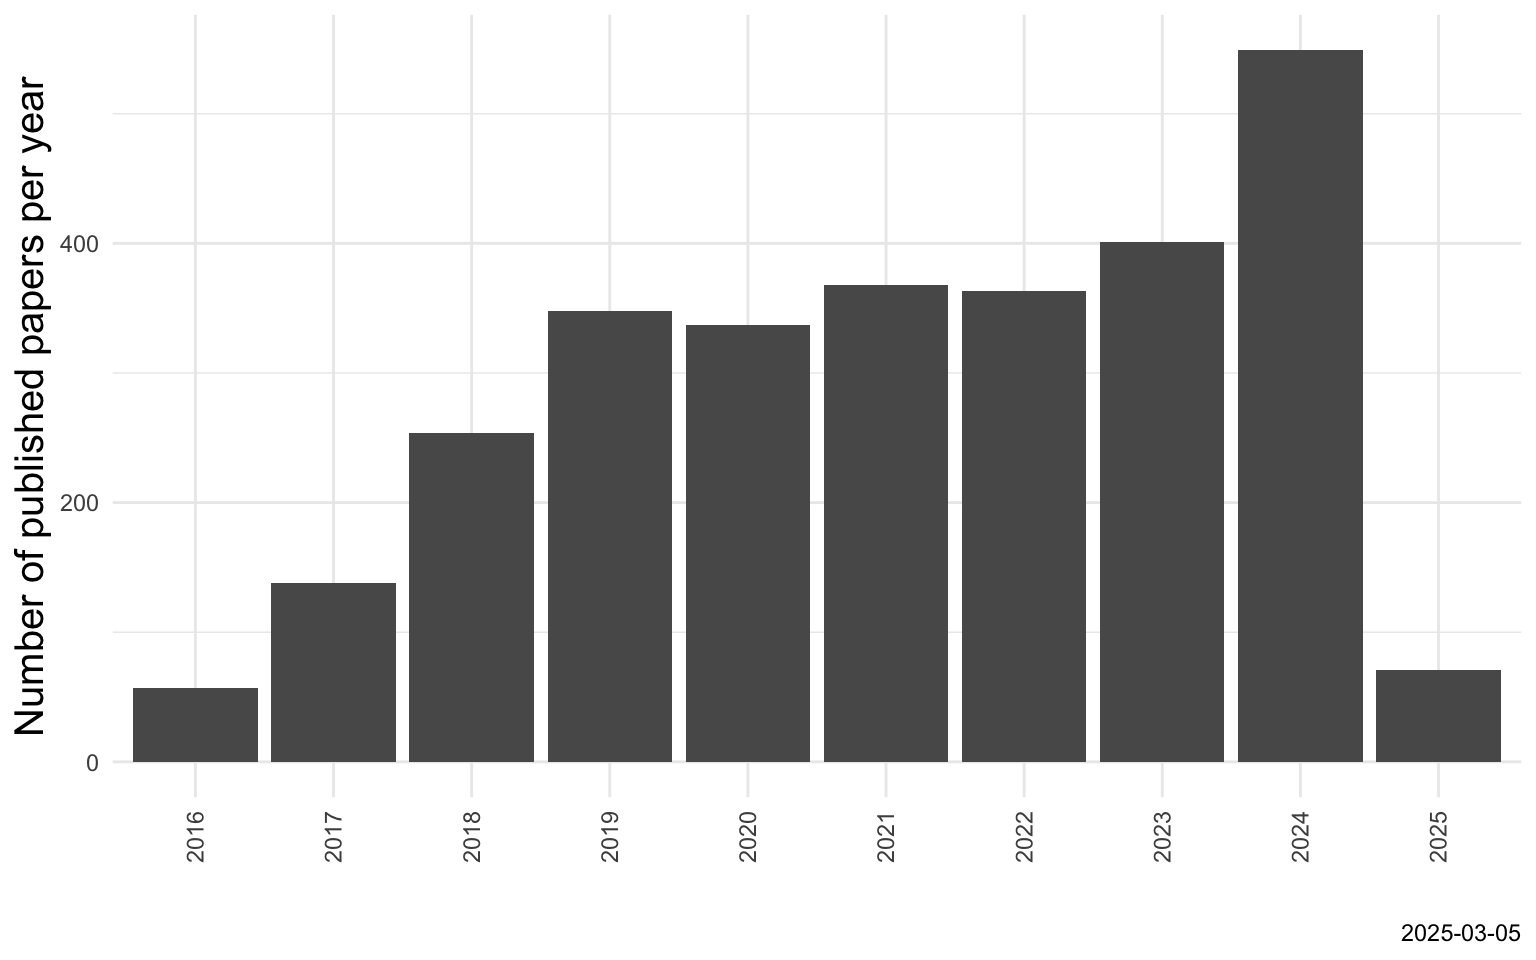
\includegraphics[width=0.35\textwidth]{joss-papers-per-year.png}
  \end{center}
  \begin{center}
    \emph{Most-cited articles}:
  \begin{tabular}{p{0.62\linewidth}@{\quad}cc}
    \textbf{Title} & \textbf{Date} & \textbf{Citations} \\
    \href{https://dx.doi.org/10.21105/joss.01686}{Welcome to the Tidyverse} & 2019-11-21 & 14\,147 \\
    \href{https://dx.doi.org/10.21105/joss.00861}{UMAP: Uniform Manifold Approximation and Projection}
    & 2018-09-02 & 6\,701 \\
    \href{https://dx.doi.org/10.21105/joss.03021}{seaborn: statistical data visualization} & 2021-04-06 & 4\,414 \\
    \href{https://dx.doi.org/10.21105/joss.03139}{performance: An R Package for Assessment, Comparison and Testing of Statistical Models} & 2021-04-21 & 2\,743 \\
    \href{https://doi.org/10.21105/joss.00772}{ggeffects: Tidy Data Frames of Marginal Effects from Regression Models} & 2018-06-29 & 1\,762 \\
  \end{tabular}
  \end{center}
}

\block{Get involved}{
 \href{https://joss.readthedocs.io/en/latest/submitting.html}{\textbf{Publish your code!}}
  JOSS is developer-friendly.  If you've already developed a significant research code
  with an open source licence, good documentation and automatic tests,
  we think it should only take an hour or two to prepare and submit your paper to JOSS.
  \begin{center}
  \qrcode{https://joss.theoj.org/}
  \end{center}
  \href{https://reviewers.joss.theoj.org/join}{\textbf{Volunteer to review!}}
  The review process is used as an opportunity to help creators improve their software.
  Reviewers are encourage to open issues and iteratively improve the software, rather
than providing a few monolithic reviews, several weeks apart.}

\column{0.5}
\block{Publication workflow}{
  \begin{center}
    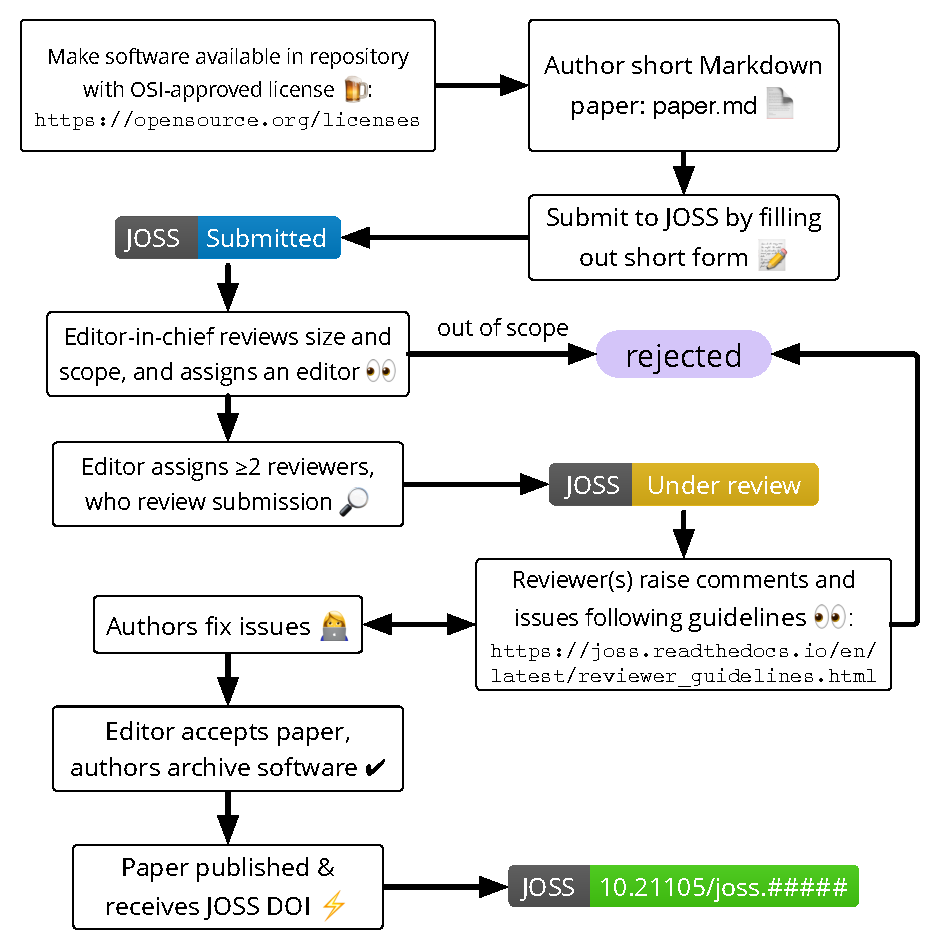
\includegraphics[width=0.42\textwidth]{JOSS-flowchart-updated-2.pdf}
  \end{center}
}

\block{Behind the scenes}
{JOSS streamlines its editorial processes by using software
  development tools.  Pre-review and review discussions happen in
  GitHub issues.  Many editorial steps are handled by the editorial
  bot: a \href{https://buffy.readthedocs.io/}{Ruby package}
  that interacts with GitHub via its API to do things
  like generate the pre-review and review issues, post checklists,
  recompile the article PDF on request, check reference DOIs, and more! \\
  \\
  Manuscripts are prepared in a flavour of Markdown and compiled to
  PDF via Pandoc.  JOSS's compilation process is available to authors
  as a GitHub action, so compliance can be checked automatically.
}

% \begin{subcolumns}
%   \subcolumn{0.45}
%   \block{JOSS homepage}{\begin{center}
%       \url{https://joss.theoj.org} \\
%       
\includegraphics[width=0.15\textwidth]{joss-qr.png}
%   \end{center}}
%   \subcolumn{0.55}
  \block{About this poster}{
Presented by Patrick Diehl and Daniel S. Katz at the \emph{3nd Annual Conference of the US Research Software Engineering Association} in Philadelphia, PA, 6--8 Oct 2025. Publication workflow diagram by Kyle Niemeyer (10.5281/zenodo.4538853). \\
%LA-UR-24-28030\\

\begin{wrapfigure}[5]{r}{10cm}\vskip-1em\includegraphics[width=\linewidth]{by.png}\end{wrapfigure}
Licensed under a Creative Commons Attribution 4.0 \\
International License: \\
\url{https://creativecommons.org/licenses/by/4.0/}
}
% \end{subcolumns}


\end{columns}

\end{document}
